% Options for packages loaded elsewhere
\PassOptionsToPackage{unicode}{hyperref}
\PassOptionsToPackage{hyphens}{url}
%
\documentclass[
]{book}
\usepackage{lmodern}
\usepackage{amsmath}
\usepackage{ifxetex,ifluatex}
\ifnum 0\ifxetex 1\fi\ifluatex 1\fi=0 % if pdftex
  \usepackage[T1]{fontenc}
  \usepackage[utf8]{inputenc}
  \usepackage{textcomp} % provide euro and other symbols
  \usepackage{amssymb}
\else % if luatex or xetex
  \usepackage{unicode-math}
  \defaultfontfeatures{Scale=MatchLowercase}
  \defaultfontfeatures[\rmfamily]{Ligatures=TeX,Scale=1}
\fi
% Use upquote if available, for straight quotes in verbatim environments
\IfFileExists{upquote.sty}{\usepackage{upquote}}{}
\IfFileExists{microtype.sty}{% use microtype if available
  \usepackage[]{microtype}
  \UseMicrotypeSet[protrusion]{basicmath} % disable protrusion for tt fonts
}{}
\makeatletter
\@ifundefined{KOMAClassName}{% if non-KOMA class
  \IfFileExists{parskip.sty}{%
    \usepackage{parskip}
  }{% else
    \setlength{\parindent}{0pt}
    \setlength{\parskip}{6pt plus 2pt minus 1pt}}
}{% if KOMA class
  \KOMAoptions{parskip=half}}
\makeatother
\usepackage{xcolor}
\IfFileExists{xurl.sty}{\usepackage{xurl}}{} % add URL line breaks if available
\IfFileExists{bookmark.sty}{\usepackage{bookmark}}{\usepackage{hyperref}}
\hypersetup{
  pdftitle={Traitement vidéo},
  pdfauthor={Guillaume Arseneault},
  hidelinks,
  pdfcreator={LaTeX via pandoc}}
\urlstyle{same} % disable monospaced font for URLs
\usepackage{longtable,booktabs}
\usepackage{calc} % for calculating minipage widths
% Correct order of tables after \paragraph or \subparagraph
\usepackage{etoolbox}
\makeatletter
\patchcmd\longtable{\par}{\if@noskipsec\mbox{}\fi\par}{}{}
\makeatother
% Allow footnotes in longtable head/foot
\IfFileExists{footnotehyper.sty}{\usepackage{footnotehyper}}{\usepackage{footnote}}
\makesavenoteenv{longtable}
\usepackage{graphicx}
\makeatletter
\def\maxwidth{\ifdim\Gin@nat@width>\linewidth\linewidth\else\Gin@nat@width\fi}
\def\maxheight{\ifdim\Gin@nat@height>\textheight\textheight\else\Gin@nat@height\fi}
\makeatother
% Scale images if necessary, so that they will not overflow the page
% margins by default, and it is still possible to overwrite the defaults
% using explicit options in \includegraphics[width, height, ...]{}
\setkeys{Gin}{width=\maxwidth,height=\maxheight,keepaspectratio}
% Set default figure placement to htbp
\makeatletter
\def\fps@figure{htbp}
\makeatother
\setlength{\emergencystretch}{3em} % prevent overfull lines
\providecommand{\tightlist}{%
  \setlength{\itemsep}{0pt}\setlength{\parskip}{0pt}}
\setcounter{secnumdepth}{5}
\usepackage{booktabs}
\usepackage{amsthm}
\makeatletter
\def\thm@space@setup{%
  \thm@preskip=8pt plus 2pt minus 4pt
  \thm@postskip=\thm@preskip
}
\makeatother
\ifluatex
  \usepackage{selnolig}  % disable illegal ligatures
\fi
\usepackage[]{natbib}
\bibliographystyle{apalike}

\title{Traitement vidéo}
\author{Guillaume Arseneault}
\date{2021-01-18}

\begin{document}
\maketitle

{
\setcounter{tocdepth}{1}
\tableofcontents
}
\hypertarget{lisez-moi}{%
\chapter{Lisez-moi}\label{lisez-moi}}

\begin{figure}
\centering
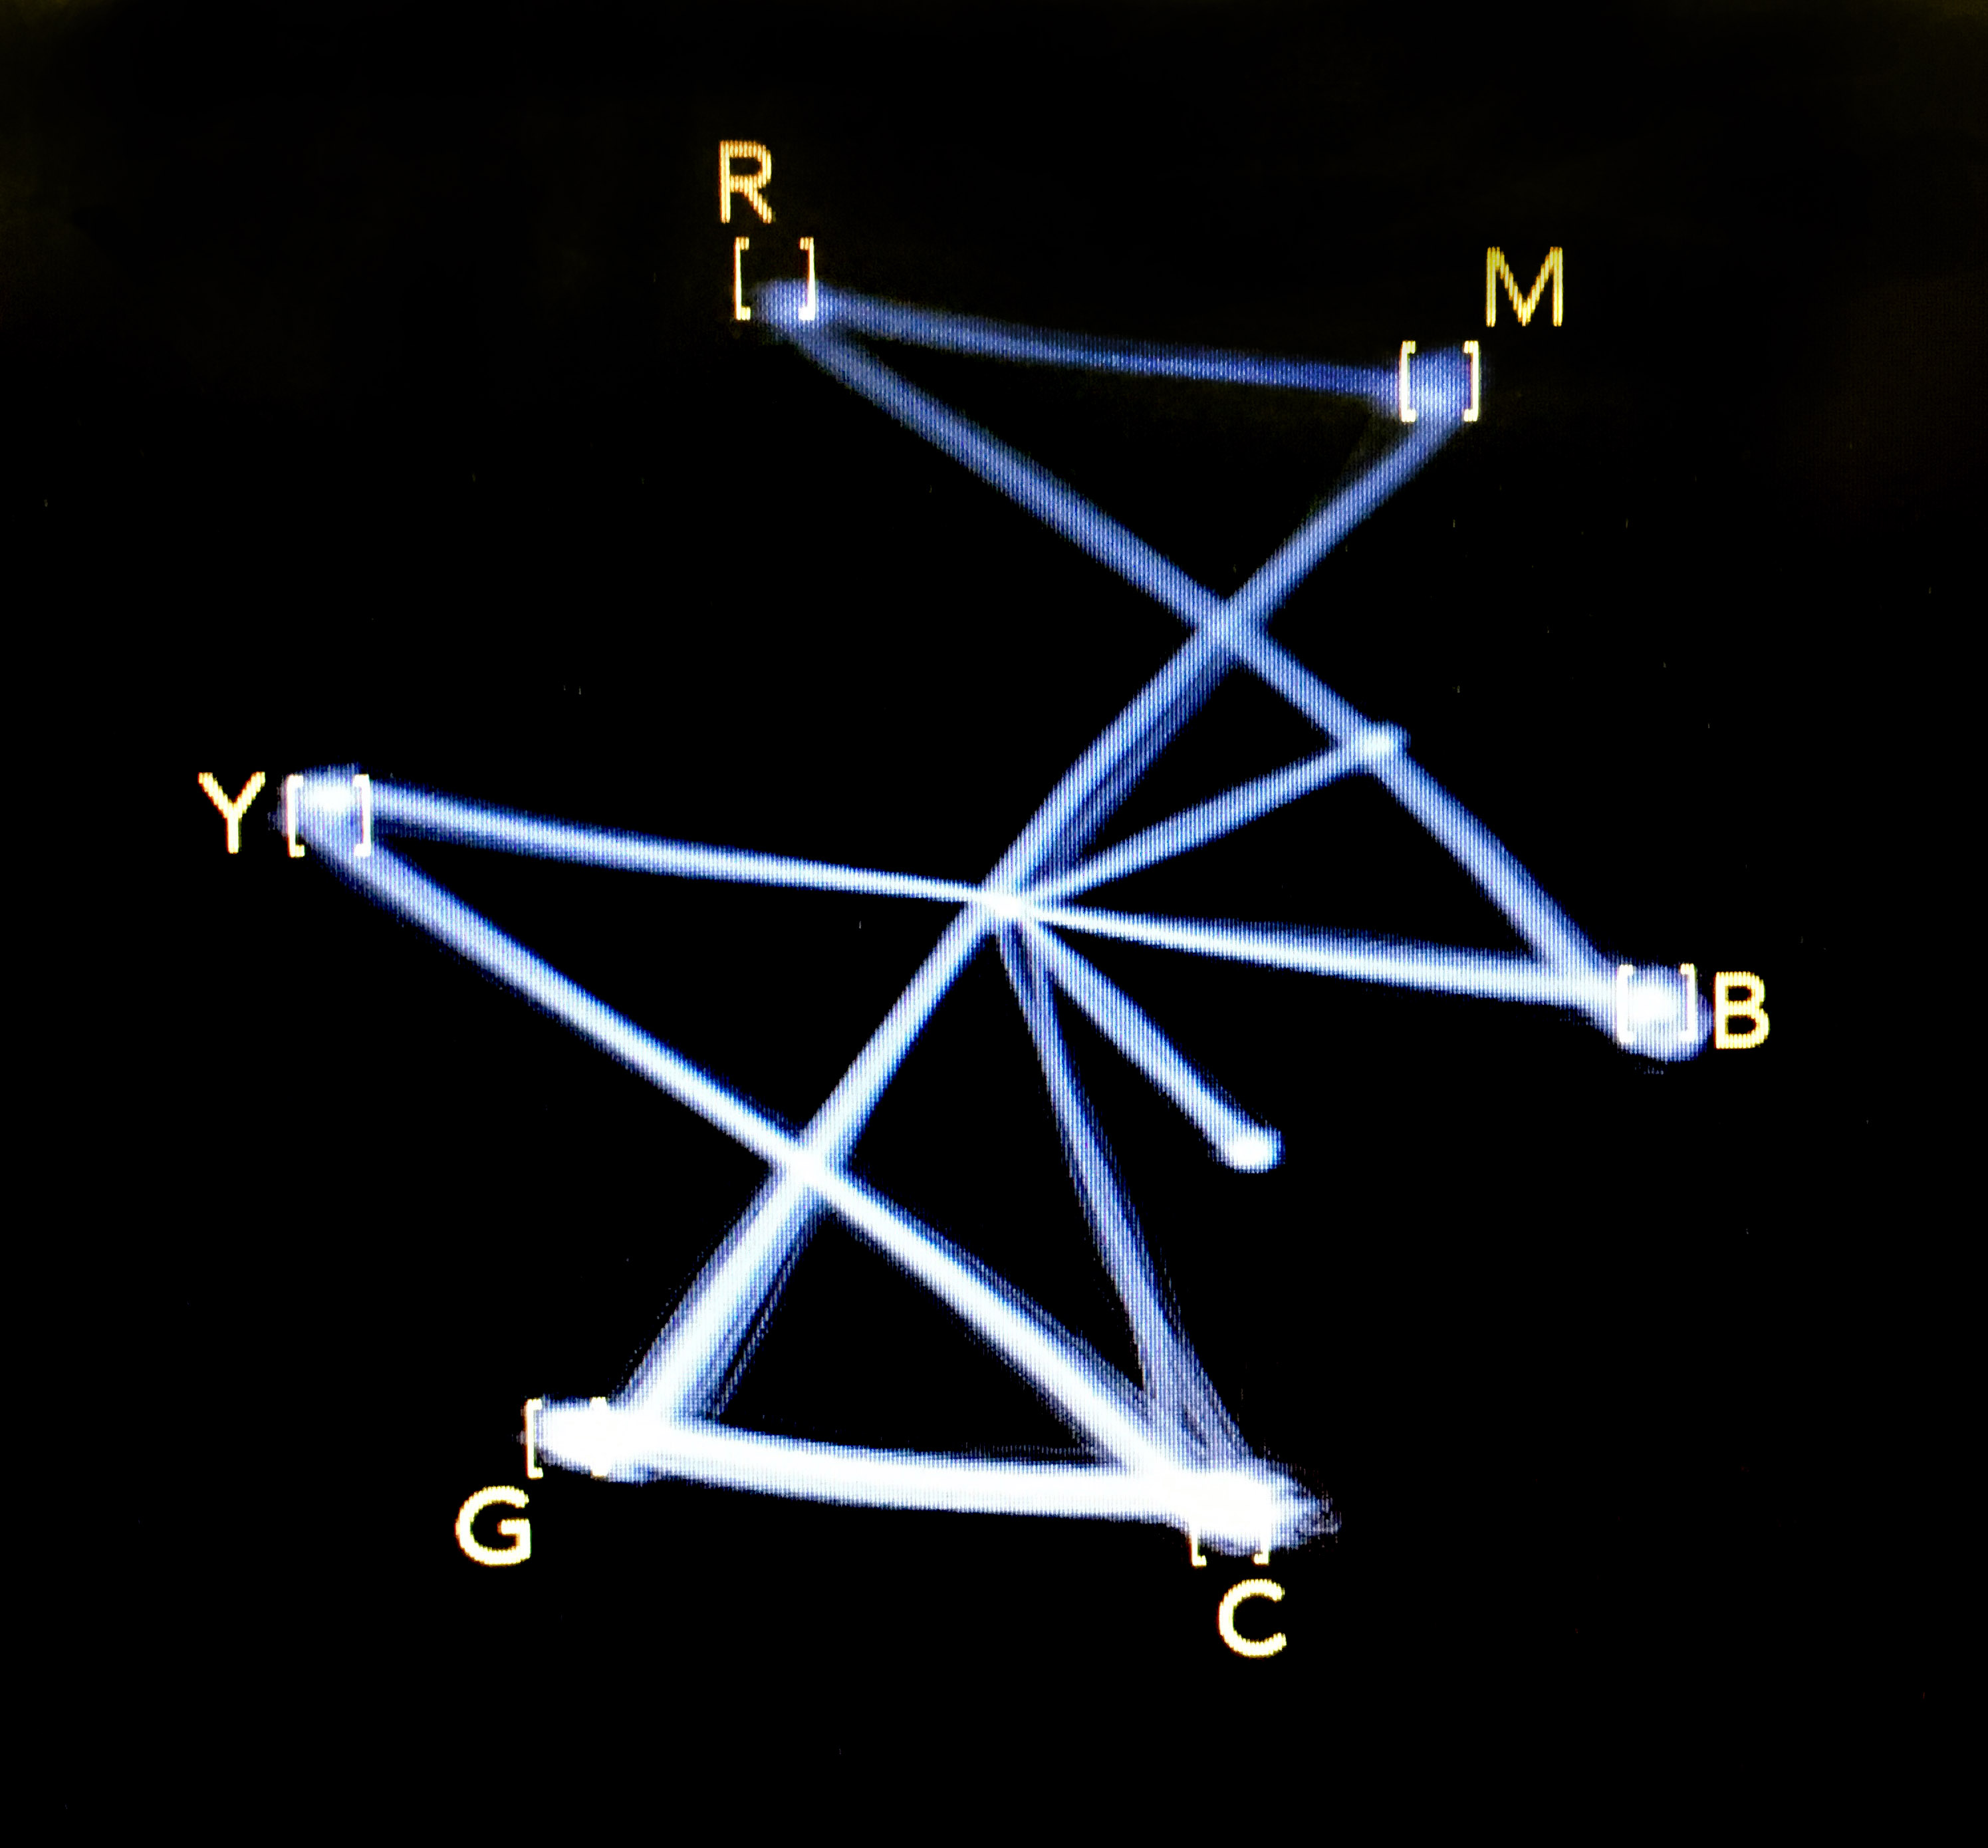
\includegraphics{images/vectorscope.jpg}
\caption{\label{fig:unnamed-chunk-1}Barres de calibration couleur sur vectorscope \citep{marsh_ColorBarsVectorscope_2016}}
\end{figure}

\hypertarget{sources}{%
\section{Sources}\label{sources}}

\begin{itemize}
\tightlist
\item
  \emph{GIT}\citep{torvalds_Git_2006} hébergé \href{https://github.com/tim-montmorency/543-traitement-video}{github.com/tim-montmorency/543-traitement-video}
\item
  \emph{Libre}\citep{stallman_GnuOrg_1983}
\item
  Écrit en \emph{RMarkdown}\citep{allaire_RmarkdownDynamicDocuments_2020}\\
\item
  Compilation via Bookdown\citep{xie_BookdownAuthoringBooks_2020}

  \begin{itemize}
  \tightlist
  \item
    \href{https://tim-montmorency.com/543-traitement-video/}{HTML}
  \item
    \href{https://tim-montmorency.com/543-traitement-video/traitement-video.pdf}{PDF}
  \item
    \href{https://tim-montmorency.com/543-traitement-video/traitement-video.epub}{EPUB}
  \end{itemize}
\item
  \href{https://github.com/tim-montmorency/543-traitement-video/blob/master/582543-traitement-video.bib}{Bibliographie Bibtex}
\end{itemize}

\hypertarget{mo-traitement-viduxe9o}{%
\chapter{582-543-MO Traitement vidéo}\label{mo-traitement-viduxe9o}}

\hypertarget{description-du-cours}{%
\section{Description du cours}\label{description-du-cours}}

\begin{itemize}
\tightlist
\item
  Techniques D'INTÉGRATION MULTIMÉDIA
\item
  Département des techniques d'intégration multimédia
\item
  582.A1
\item
  Pondération : 1-2-2
\item
  Unités: 1,66
\item
  Heures-contact : 45
\item
  Session : 4
\end{itemize}

Ce cours permet à l'étudiante ou l'étudiant d'enregistrer, de modifier et de traiter des images en temps réel.
L'étudiant sera appelé à appliquer des effets visuels aux images vidéo et à adapter les images en fonction de l'intégration.

\hypertarget{objectifs}{%
\section{Objectifs}\label{objectifs}}

\hypertarget{intuxe9grateur-et-ministuxe9riel}{%
\subsection{Intégrateur et ministériel}\label{intuxe9grateur-et-ministuxe9riel}}

\begin{itemize}
\tightlist
\item
  015J Traiter les images en mouvement
\end{itemize}

\hypertarget{apprentissages}{%
\subsection{Apprentissages}\label{apprentissages}}

\begin{itemize}
\tightlist
\item
  Adapter l'images en mouvement (Importance relative\,: 40\% )
\item
  Programmer des effets visuels interactifs (Importance relative\,: 40\% )
\item
  Intégrer l'image en mouvement interactive à une production médiatique (Importance relative\,: 20\% )
\end{itemize}

\hypertarget{duxe9veloppement}{%
\section{Développement}\label{duxe9veloppement}}

\hypertarget{attitudes-professionnelles}{%
\subsection{Attitudes professionnelles}\label{attitudes-professionnelles}}

\begin{itemize}
\tightlist
\item
  Curiosité
\item
  Capacité de partage
\item
  Créativité
\item
  Esprit critique
\item
  Sens esthétique
\end{itemize}

\hypertarget{habiletuxe9s-transdisciplinaires}{%
\subsection{Habiletés transdisciplinaires}\label{habiletuxe9s-transdisciplinaires}}

\begin{itemize}
\tightlist
\item
  Profil \textbf{technologies de l'information et de la communication (TIC)}
\item
  Les étudiantes et étudiants auront à exploiter les TIC de manière efficace et responsable.
\item
  Recherche, traitement et présentation de l'information.
\end{itemize}

\hypertarget{pruxe9alables}{%
\section{Préalables}\label{pruxe9alables}}

\hypertarget{pruxe9alable-absolu-au-pruxe9sent-cours}{%
\subsection{Préalable absolu au présent cours~:}\label{pruxe9alable-absolu-au-pruxe9sent-cours}}

\begin{itemize}
\tightlist
\item
  582 413 MO Montage vidéo
\end{itemize}

\hypertarget{pruxe9alable-absolu-aux-cours-suivants}{%
\subsection{Préalable absolu aux cours suivants~:}\label{pruxe9alable-absolu-aux-cours-suivants}}

\begin{itemize}
\tightlist
\item
  582~513 MO Conception de projet multimédia
\item
  582 66B MO Expérience multimédia interactive
\item
  582 66G MO Production Web en entreprise
\end{itemize}

\hypertarget{contexte-particulier-dapprentissage}{%
\section{Contexte particulier d'apprentissage}\label{contexte-particulier-dapprentissage}}

\begin{itemize}
\tightlist
\item
  À distance; synchrone.
\item
  Possibilité d'utiliser le laboratoire informatique et le studio.
\end{itemize}

\hypertarget{fiche-technique}{%
\subsection{Fiche technique}\label{fiche-technique}}

\begin{itemize}
\tightlist
\item
  Ordinateurs, projecteurs à haute luminosité ou télévision, haut-parleurs professionnels, casque audio, et tout le matériel disponible pour TIM
\item
  Logiciels de montage vidéo et traitemet vidéo en temps réel
\item
  Languages et protocoles de paramétrage\\
\item
  Technicienne ou technicien en travaux pratiques
\end{itemize}

\hypertarget{contenus_essentiels}{%
\section{Contenus essentiels}\label{contenus_essentiels}}

\hypertarget{survol-historique}{%
\subsection{Survol historique}\label{survol-historique}}

\begin{itemize}
\tightlist
\item
  \protect\hyperlink{evolution_historique}{Évolution historique du traitement vidéo dans les différentes formes d'art}

  \begin{itemize}
  \tightlist
  \item
    \protect\hyperlink{evolution_historique_performance}{Performance}
  \item
    \protect\hyperlink{evolution_historique_installation}{Installation}
  \item
    \protect\hyperlink{evolution_historique_technologies}{Évolution des technologies associées}
  \end{itemize}
\item
  \protect\hyperlink{evolution_historique_language}{Langages et moyens expressifs de l'image en mouvement}
\end{itemize}

\hypertarget{fondements-technique}{%
\subsection{Fondements technique}\label{fondements-technique}}

\begin{itemize}
\tightlist
\item
  \protect\hyperlink{lexique_fichiers}{Formats de fichiers}
\item
  \protect\hyperlink{lexique_encodage}{Encodage des vidéos}\\
\item
  \protect\hyperlink{aquerir_captation}{Captation vidéo en temps réel}
\item
  \protect\hyperlink{traiter_logiciels}{Logiciels de traitement vidéo en temps réel et d'interactivité}
\item
  \protect\hyperlink{programmer_logiciels}{Logiciels de programmation nodale}
\item
  Notions de traitement vidéo

  \begin{itemize}
  \tightlist
  \item
    pixels
  \item
    couleurs
  \item
    texture
  \item
    matrice
  \item
    mémoire tampon
  \item
    alpha channel
  \item
    rendu OpenGL
  \end{itemize}
\end{itemize}

\hypertarget{traitement-de-limages-en-mouvement}{%
\subsection{Traitement de l'images en mouvement}\label{traitement-de-limages-en-mouvement}}

\begin{itemize}
\tightlist
\item
  Usage de capture vidéo en temps réel\\
\item
  Effets visuels et filtres applicables en temps réel sur des matériaux visuels\\
\item
  Traitement visuel en temps réel à l'aide d'effets et de logiciels de programmation multimédia et nodale
\item
  Flot de données entre les objets du logiciel
\item
  Exploitation des fonctions des logiciels de traitement vidéo en temps réel
\item
  Utilisation de nuanceurs (shaders)
\end{itemize}

\hypertarget{programmation-deffets-visuels}{%
\subsection{Programmation d'effets visuels}\label{programmation-deffets-visuels}}

\begin{itemize}
\tightlist
\item
  Programmation de compositions visuelles génératives
\item
  Réalisation d'un échantillonneur/mixeur visuel
\item
  Programmation pour contrôler la lecture vidéo,

  \begin{itemize}
  \tightlist
  \item
    montage temps réel
  \item
    niveau des couleurs
  \item
    alpha channel\\
  \end{itemize}
\item
  Programmation nodale pour créer des effets en temps réel

  \begin{itemize}
  \tightlist
  \item
    position
  \item
    rotation
  \item
    dimensions
  \item
    mixage d'images
  \item
    incrustation
  \item
    distorsion
  \item
    délais
  \item
    rétroaction (feedback)
  \item
    modification de couleurs
  \item
    chromakey
  \item
    lumière
  \item
    fumée
  \item
    texture
  \end{itemize}
\item
  Nuanceurs (shaders)\,: vertex, pixel et géométrie
\end{itemize}

\hypertarget{image-en-mouvement-et-interactivituxe9}{%
\subsection{Image en mouvement et interactivité}\label{image-en-mouvement-et-interactivituxe9}}

\begin{itemize}
\tightlist
\item
  Intégration des composantes dans une production interactive
\item
  Configuration logicielle et matérielle d'une production interactive\\
\item
  Conceptualisation et scénarisation d'un projet visuel interactif\\
\item
  Captation de mouvement et de présence
\item
  Programmation de la captation de mouvement et de présence
\item
  Utilisation d'interfaces de contrôle interactives
\item
  Utilisation d'OSC, MIDI, DMX ou ArtNet pour interagir avec d'autre logiciels et interfaces de contrôle
\end{itemize}

\hypertarget{gestion-de-projets}{%
\subsection{Gestion de projets}\label{gestion-de-projets}}

\begin{itemize}
\tightlist
\item
  Schématisation
\item
  Prototypage
\item
  Gestion de banques d'images
\item
  Optimisation des performances de l'application
\item
  Test de contrôle de qualité
\item
  Préréglages
\item
  Optimisation de la programmation et commentaires
\item
  Console de débogage
\item
  Exportation de projets
\item
  Formats de sauvegarde\\
\item
  Application autonome
\item
  Sauvegarde et archivage des médias
\item
  Ajustement des effets visuels en fonction des tests
\end{itemize}

\hypertarget{calendrier}{%
\chapter{Calendrier}\label{calendrier}}

\href{https://www.cmontmorency.qc.ca/wp-content/uploads/images/college/administration/CALENDRIER-SCOLAIRE-2020-2021.pdf}{Calendrier Collège Montmorency 2020-2021}

\begin{table}

\caption{\label{tab:calendrier}Calendrier}
\centering
\begin{tabular}[t]{lll}
\toprule
SÉANCE & CONTENU ABORDÉ EN CLASSE ET OBJECTIF & ACTIVITÉS AUTONOME\\
\midrule
1; 3 février & plan de cour, [historique du traitement vidéo](\#evolution\_historique) & 1 aa\\
2; 10 février & [composantes du signal vidéo](\#lexique\_composantes) & Préparation [evaluation 1](\#evaluation\_1)\\
3; 17 février & Formatif:Approbation des sujet [evaluation 1](\#evaluation\_1) & Préparation [evaluation 1](\#evaluation\_1)\\
4; 24 février & Remise [évaluation\_1](\#evaluation\_1) & Préparation [evaluation 2](\#evaluation\_2)\\
X ; 3 mars & Journées de rattrapage (Pas de cours) & Préparation [evaluation 2](\#evaluation\_2)\\
\addlinespace
5; 10 mars & Remise [évaluation\_2](\#evaluation\_2) & \\
6; 17 mars &  & Compléter [évaluation\_3](\#evaluation\_3)\\
7; 24 mars & 8e & 8 aa\\
8; 31 mars & Remise [évaluation\_4](\#evaluation\_4) & 9 aa\\
X; 7 avril & Congé (Pas de cours) & 10 aa\\
\addlinespace
9; 14 avril & 11e & Préparation [évaluation\_5](\#evaluation\_5)\\
10; 21 avril & Remise [évaluation\_5](\#evaluation\_5) & 12 aa\\
11; 28 avril & 13e & 13 aa\\
12; 5 mai & 14e & 14 aa\\
13; 12 mai & Préparation [évaluation\_6](\#evaluation\_6) & Préparation [évaluation\_6](\#evaluation\_6)\\
\addlinespace
X; 19 mai & épreuve uniforme de français (Pas de cours) & \\
14; 25 mai & Remise [évaluation\_6](\#evaluation\_6) & \\
\bottomrule
\end{tabular}
\end{table}

\hypertarget{exercices}{%
\chapter{Exercices}\label{exercices}}

\hypertarget{formatif_1}{%
\section{Approbation du sujet pour le corpus vidéo}\label{formatif_1}}

\hypertarget{formatif}{%
\subsection{Formatif}\label{formatif}}

\hypertarget{sommatif_1}{%
\section{Corpus vidéo}\label{sommatif_1}}

\hypertarget{sommatif-15-individuel}{%
\subsection{Sommatif 15\% individuel}\label{sommatif-15-individuel}}

\hypertarget{pruxe9sentation-orale-individuelle-de-type-partage-duxe9cran-de-5-minutes}{%
\subsection{Présentation orale individuelle de type partage d'écran de \textasciitilde5 minutes}\label{pruxe9sentation-orale-individuelle-de-type-partage-duxe9cran-de-5-minutes}}

\begin{itemize}
\tightlist
\item
  Traiter une oeuvre et/ou une technique en lien avec le traitement vidéo\\
\item
  Partager un extrait court et des capture écran si approprié
\item
  Présenter son contexte artistique et historique ainsi que les techniques et technologies employées
\item
  Sugérer une technique actuelle pour reproduire le résultat visuel
\item
  Tenter de lier des \protect\hyperlink{contenus_essentiels}{contenus essentiels} à la présentation
\end{itemize}

\hypertarget{formatif_2}{%
\section{Présentation d'une question}\label{formatif_2}}

\hypertarget{formatif-1}{%
\subsection{Formatif}\label{formatif-1}}

\hypertarget{sommatif_2}{%
\section{Question quiz}\label{sommatif_2}}

\hypertarget{individuel}{%
\subsection{10\% individuel}\label{individuel}}

\hypertarget{ruxe9daction-dune-question-pertinant-et-originale-pour-le-quiz}{%
\subsection{Rédaction d'une question pertinant et originale pour le quiz}\label{ruxe9daction-dune-question-pertinant-et-originale-pour-le-quiz}}

\begin{itemize}
\tightlist
\item
  Rédaction d'une question théorique originale portant sur la matière du cours
\item
  Se référer aux \protect\hyperlink{contenus_essentiels}{contenus essentiels}
\item
  4 choix de réponses éloquents comprenant la réponse
\end{itemize}

\hypertarget{sommatif_3}{%
\section{Quiz théorique}\label{sommatif_3}}

\hypertarget{individuel-1}{%
\subsection{15\% individuel}\label{individuel-1}}

\begin{itemize}
\tightlist
\item
  formulaire en ligne à répondre individuellement
\item
  Contient les questions quiz des deux groupes ainsi ceux de l'enseignement
\end{itemize}

\hypertarget{sommatif_4}{%
\section{Scènes vidéo}\label{sommatif_4}}

\hypertarget{individuel-2}{%
\subsection{15\% individuel}\label{individuel-2}}

\hypertarget{partage-duxe9cran-individuelle-5-minutes}{%
\subsection{Partage d'écran individuelle \textasciitilde5 minutes}\label{partage-duxe9cran-individuelle-5-minutes}}

\begin{itemize}
\tightlist
\item
  Palette de 8 scène

  \begin{itemize}
  \tightlist
  \item
    échantillons vidéo
  \item
    caméra vidéo
  \item
    source html
  \item
    source nuancier
  \item
    etc.
  \end{itemize}
\end{itemize}

\hypertarget{sommatif_5}{%
\section{Mélangeur vidéo interactif}\label{sommatif_5}}

\hypertarget{individuel-3}{%
\subsection{15\% individuel}\label{individuel-3}}

\hypertarget{partage-duxe9cran-individuelle-5-minutes-1}{%
\subsection{Partage d'écran individuelle \textasciitilde5 minutes}\label{partage-duxe9cran-individuelle-5-minutes-1}}

\begin{itemize}
\tightlist
\item
  Variation temps réel des paramètres vidéo programmées
\end{itemize}

\hypertarget{sommatif_6}{%
\section{Installation interactive et/ou performance audiovisuel}\label{sommatif_6}}

\hypertarget{individuel-uxe9quipe-et-classe.}{%
\subsection{25\% individuel, équipe et classe.}\label{individuel-uxe9quipe-et-classe.}}

\hypertarget{pruxe9sentation-de-type-fluxstream-video-de-lensemble-des-projets}{%
\subsection{Présentation de type Flux(Stream) video de l'ensemble des projets}\label{pruxe9sentation-de-type-fluxstream-video-de-lensemble-des-projets}}

où le traitement vidéo est effectué en temps réel
* Présentation de type partage d'écran et stream simultané
* Changement de scène
* Changement de paramètres asservie
* Pourrait prendre la forme d'un VJ set via scènes dans OBS

\hypertarget{historique}{%
\chapter{Historique du traitement vidéo}\label{historique}}

\hypertarget{evolution_historique}{%
\section{Évolution historique du traitement vidéo dans les différentes formes d'art}\label{evolution_historique}}

\hypertarget{evolution_historique_performance}{%
\subsection{Performance}\label{evolution_historique_performance}}

\hypertarget{evolution_historique_installation}{%
\subsection{Installation}\label{evolution_historique_installation}}

\hypertarget{evolution_historique_technologies}{%
\subsection{Évolution des technologies associées}\label{evolution_historique_technologies}}

\hypertarget{evolution_historique_language}{%
\section{Langages et moyens expressifs de l'image en mouvement}\label{evolution_historique_language}}

\hypertarget{lexique}{%
\chapter{Lexique technique et technologique}\label{lexique}}

\hypertarget{lexique_composantes}{%
\section{Composantes du signal vidéo}\label{lexique_composantes}}

\hypertarget{signaux-de-transmission}{%
\subsection{Signaux de transmission}\label{signaux-de-transmission}}

\begin{itemize}
\tightlist
\item
  \href{https://en.wikipedia.org/wiki/Video\#Analog_video}{Signaux analogues/digitaux}

  \begin{itemize}
  \tightlist
  \item
    \href{https://en.wikipedia.org/wiki/Analog_television}{transmission télévisuelle analogue}
  \end{itemize}
\end{itemize}

\hypertarget{ruxe9solutions}{%
\subsection{résolutions}\label{ruxe9solutions}}

\begin{itemize}
\tightlist
\item
  \href{https://en.wikipedia.org/wiki/Computer_display_standard\#/media/File:Vector_Video_Standards2.svg}{résolutions}
\end{itemize}

\hypertarget{ratio}{%
\subsection{Ratio}\label{ratio}}

\begin{itemize}
\tightlist
\item
  \href{https://en.wikipedia.org/wiki/Display_aspect_ratio}{ratios image}
\item
  \href{https://en.wikipedia.org/wiki/Pixel_aspect_ratio}{ratios-pixels}
\end{itemize}

\hypertarget{duxe9bit}{%
\subsection{Débit}\label{duxe9bit}}

\begin{itemize}
\tightlist
\item
  \href{https://en.wikipedia.org/wiki/Bit_rate\#Video}{Débit (bitrate)}
\end{itemize}

\hypertarget{uxe9chantillonnage}{%
\subsection{Échantillonnage}\label{uxe9chantillonnage}}

\begin{itemize}
\tightlist
\item
  Profondeur de l'échantillonnage couleur

  \begin{itemize}
  \tightlist
  \item
    \href{https://en.wikipedia.org/wiki/Color_depth}{bit/canal}\\
  \end{itemize}
\item
  \href{https://en.wikipedia.org/wiki/Chroma_subsampling\#Sampling_systems_and_ratios}{chroma subsampling}

  \begin{itemize}
  \tightlist
  \item
    \href{https://upload.wikimedia.org/wikipedia/commons/0/06/Colorcomp.jpg}{4:4:4 vs 4:2:2 vs 4:2:0}
  \item
    \href{https://en.wikipedia.org/wiki/Alpha_compositing}{4:4:4 vs 4:4:4:4}
  \end{itemize}
\end{itemize}

\hypertarget{cadence}{%
\subsection{Cadence}\label{cadence}}

\begin{itemize}
\tightlist
\item
  \href{https://frames-per-second.appspot.com}{Cadence}
\end{itemize}

\hypertarget{trame}{%
\subsection{Trame}\label{trame}}

\begin{itemize}
\tightlist
\item
  \href{https://web.archive.org/web/20140222010640/http://neuron2.net/LVG/interlacing.html}{Trame (progressif/entrelacé)}
\end{itemize}

\hypertarget{poid}{%
\subsection{Poid}\label{poid}}

\begin{itemize}
\tightlist
\item
  \href{https://toolstud.io/video/filesize.php?imagewidth=1920\&imageheight=1080\&framerate=29.97\&timeduration=60\&timeunit=seconds}{calcul de grosseur de fichier}
\item
  \href{https://toolstud.io/video/bitrate.php?imagewidth=1\&imageheight=1\&colordepth=24\&framerate=29.97}{calcul de bitrate}
\end{itemize}

\hypertarget{lexique_fichiers}{%
\section{Formats de fichiers}\label{lexique_fichiers}}

\hypertarget{containers}{%
\subsection{Containers}\label{containers}}

\begin{longtable}[]{@{}ll@{}}
\toprule
nom & extension\tabularnewline
\midrule
\endhead
QuickTime & .mov\tabularnewline
Matroska & .mkv\tabularnewline
Mpeg4 & .mp4\tabularnewline
Windows Media Video & .wmv\tabularnewline
Audio Video Interleaved & .avi\tabularnewline
Theora & .ogv\tabularnewline
\bottomrule
\end{longtable}

\href{https://en.wikipedia.org/wiki/Comparison_of_video_container_formats}{wiki:Comparison\_of\_video\_container\_formats}

\hypertarget{codecs}{%
\subsection{Codecs}\label{codecs}}

\begin{longtable}[]{@{}lll@{}}
\toprule
Codec & compression & usage\tabularnewline
\midrule
\endhead
H.264\&VP8 & intra \& inter & lecture\textless1080p\tabularnewline
HEVC\&VP9 & intra \& inter & lecture\textless4k\tabularnewline
proRes & intra & montage\tabularnewline
dnxHD & intra & montage\tabularnewline
HAP & intra & GPU\&SSD\tabularnewline
\bottomrule
\end{longtable}

\hypertarget{lexique_encodage}{%
\section{Encodage vidéo}\label{lexique_encodage}}

\hypertarget{compression}{%
\subsection{compression}\label{compression}}

\hypertarget{losslesslossy}{%
\subsubsection{lossless/lossy}\label{losslesslossy}}

\hypertarget{encodage-viduxe9o-sans-perte---lossless}{%
\paragraph{\texorpdfstring{\href{https://en.wikipedia.org/wiki/List_of_codecs\#Lossless_video_compression}{Encodage vidéo sans perte - lossless}}{Encodage vidéo sans perte - lossless}}\label{encodage-viduxe9o-sans-perte---lossless}}

\begin{itemize}
\tightlist
\item
  Apple Animation (QuickTime RLE)
\item
  CinemaDNG Raw (Adobe, Blackmagic)
\item
  séquence d'images (tiff, openexr)
\end{itemize}

\hypertarget{encodage-viduxe9o-avec-perte--lossy}{%
\paragraph{\texorpdfstring{\href{https://en.wikipedia.org/wiki/List_of_codecs\#Lossy_compression_2}{Encodage vidéo avec perte -lossy}}{Encodage vidéo avec perte -lossy}}\label{encodage-viduxe9o-avec-perte--lossy}}

\begin{itemize}
\tightlist
\item
  H.264\&VP8
\item
  HEVC\&VP9
\item
  proRes, dnxHD, cineform\\
\item
  HAP \& HAPQ
\end{itemize}

\hypertarget{intrainter-frame}{%
\subsubsection{intra/inter frame}\label{intrainter-frame}}

\hypertarget{intraframe}{%
\paragraph{intraframe}\label{intraframe}}

\begin{itemize}
\tightlist
\item
  Toute l'image individuellement compressée dans chaque image.

  \begin{itemize}
  \tightlist
  \item
    prores, dnxHD, photoJpeg, Apple intermediate codec (aic), cineform
  \end{itemize}
\end{itemize}

\hypertarget{interframe}{%
\paragraph{\texorpdfstring{\href{https://en.wikipedia.org/wiki/Inter_frame}{interframe}}{interframe}}\label{interframe}}

\begin{itemize}
\tightlist
\item
  image temporellement compressée, \href{http://dvd-hq.info/data_compression_3.php}{ce qui change}

  \begin{itemize}
  \tightlist
  \item
    \href{https://en.wikipedia.org/wiki/Video_compression_picture_types}{images: I (clef), P (\textless-) et B(\textless-\textgreater)}
  \item
    \href{https://en.wikipedia.org/wiki/Inter_frame\#/media/File:IPB_images_sequence.png}{GOP : group of picture}
  \end{itemize}
\item
  usage créatif \href{https://www.youtube.com/watch?v=rMSsw4CZvKg}{1}, \href{https://www.youtube.com/watch?v=rSmEOk5AiN0}{2}, \href{https://www.youtube.com/watch?v=dNa0-xrKi3Q}{3}
\end{itemize}

pour des usages réguliers voir :

\begin{itemize}
\tightlist
\item
  FFmpeg Cookbook for Archivists \citep{kromer_FFmpegCookbookArchivists_2020}
\item
  FFmpeg Cookbook par Greg Wessels \citep{wessels_FFmpegCookbook_2017}
\end{itemize}

pour usages artistiques :

\begin{itemize}
\tightlist
\item
  FFmpeg artschool \citep{associationofmovingimagearchivists_FFmpegArtschool_2020}
\end{itemize}

\hypertarget{aquerir}{%
\chapter{Aquérir l'image en mouvement}\label{aquerir}}

\hypertarget{aquerir_captation}{%
\section{Captation vidéo en temps réel}\label{aquerir_captation}}

\hypertarget{captation-de-mouvement-et-de-pruxe9sence}{%
\section{Captation de mouvement et de présence}\label{captation-de-mouvement-et-de-pruxe9sence}}

\hypertarget{usages-de-capture-viduxe9o-temps-ruxe9el}{%
\section{Usages de capture vidéo temps réel}\label{usages-de-capture-viduxe9o-temps-ruxe9el}}

\hypertarget{traiter}{%
\chapter{Traiter l'image en mouvement}\label{traiter}}

\hypertarget{traiter_logiciels}{%
\section{Logiciels de traitement vidéo en temps réel et d'interactivité}\label{traiter_logiciels}}

\begin{itemize}
\tightlist
\item
  Open Broadcast Studio
\item
  ffmpeg
\end{itemize}

\hypertarget{notions-de-traitement-viduxe9o}{%
\section{Notions de traitement vidéo}\label{notions-de-traitement-viduxe9o}}

\hypertarget{pixels}{%
\subsection{Pixels}\label{pixels}}

\hypertarget{couleurs}{%
\subsection{Couleurs}\label{couleurs}}

\hypertarget{texture}{%
\subsection{Texture}\label{texture}}

\hypertarget{matrice}{%
\subsection{Matrice}\label{matrice}}

\hypertarget{muxe9moire-tampon}{%
\subsection{Mémoire tampon}\label{muxe9moire-tampon}}

\hypertarget{alpha-channel}{%
\subsection{Alpha channel}\label{alpha-channel}}

\hypertarget{rendu-opengl}{%
\subsection{Rendu OpenGL}\label{rendu-opengl}}

\hypertarget{traitement-visuel-en-temps-ruxe9el-uxe0-laide-deffets-et-de-logiciels-de-programmation-multimuxe9dia-et-nodale}{%
\section{Traitement visuel en temps réel à l'aide d'effets et de logiciels de programmation multimédia et nodale}\label{traitement-visuel-en-temps-ruxe9el-uxe0-laide-deffets-et-de-logiciels-de-programmation-multimuxe9dia-et-nodale}}

\hypertarget{exploitation-des-fonctions-des-logiciels-de-traitement-viduxe9o-en-temps-ruxe9el}{%
\section{Exploitation des fonctions des logiciels de traitement vidéo en temps réel}\label{exploitation-des-fonctions-des-logiciels-de-traitement-viduxe9o-en-temps-ruxe9el}}

\hypertarget{effets-visuels-et-filtres-applicables-en-temps-ruxe9el-sur-des-matuxe9riaux-visuels}{%
\section{Effets visuels et filtres applicables en temps réel sur des matériaux visuels}\label{effets-visuels-et-filtres-applicables-en-temps-ruxe9el-sur-des-matuxe9riaux-visuels}}

\hypertarget{flot-de-donnuxe9es-entre-les-objets-du-logiciel}{%
\section{Flot de données entre les objets du logiciel}\label{flot-de-donnuxe9es-entre-les-objets-du-logiciel}}

\hypertarget{utilisation-de-nuanciers-shaders}{%
\section{Utilisation de nuanciers (shaders)}\label{utilisation-de-nuanciers-shaders}}

\hypertarget{programmer}{%
\chapter{Programmer des effets visuels}\label{programmer}}

\hypertarget{logiciels-de-programmation-nodaleprogrammer_logiciels}{%
\section{Logiciels de programmation nodale\{programmer\_logiciels\}}\label{logiciels-de-programmation-nodaleprogrammer_logiciels}}

\begin{itemize}
\tightlist
\item
  Pure Data
\item
  Pure Data et Open Broadcast Studio
\item
  Pure Data et Ofelia
\end{itemize}

\hypertarget{ruxe9alisation-dun-uxe9chantillonneurmuxe9langeur-visuel}{%
\section{Réalisation d'un échantillonneur/mélangeur visuel}\label{ruxe9alisation-dun-uxe9chantillonneurmuxe9langeur-visuel}}

\hypertarget{montage-temps-ruxe9el}{%
\section{Montage temps réel}\label{montage-temps-ruxe9el}}

\hypertarget{contruxf4ler-de-la-tuxeate-de-lecture-viduxe9o}{%
\subsection{Contrôler de la tête de lecture vidéo}\label{contruxf4ler-de-la-tuxeate-de-lecture-viduxe9o}}

\hypertarget{position}{%
\subsubsection{Position}\label{position}}

\hypertarget{boucle}{%
\subsubsection{Boucle}\label{boucle}}

\hypertarget{vitesse}{%
\subsubsection{Vitesse}\label{vitesse}}

\hypertarget{programmation-deffets-temps-ruxe9el}{%
\section{Programmation d'effets temps réel}\label{programmation-deffets-temps-ruxe9el}}

\hypertarget{position-1}{%
\subsection{Position}\label{position-1}}

\hypertarget{rotation}{%
\subsection{Rotation}\label{rotation}}

\hypertarget{dimensions}{%
\subsection{Dimensions}\label{dimensions}}

\hypertarget{niveau-des-couleurs}{%
\subsection{Niveau des couleurs}\label{niveau-des-couleurs}}

\hypertarget{alpha-channel-1}{%
\subsection{Alpha channel}\label{alpha-channel-1}}

\hypertarget{modification-de-couleurs}{%
\subsection{Modification de couleurs}\label{modification-de-couleurs}}

\hypertarget{mixage-dimages}{%
\subsection{Mixage d'images}\label{mixage-dimages}}

\hypertarget{incrustation}{%
\subsection{Incrustation}\label{incrustation}}

\hypertarget{chromakey}{%
\subsection{chromakey}\label{chromakey}}

\hypertarget{distorsion}{%
\subsection{Distorsion}\label{distorsion}}

\hypertarget{duxe9lais}{%
\subsection{Délais}\label{duxe9lais}}

\hypertarget{ruxe9troaction-feedback}{%
\subsection{Rétroaction (feedback)}\label{ruxe9troaction-feedback}}

\hypertarget{nuanceurs-shaders}{%
\section{Nuanceurs (shaders)\,:}\label{nuanceurs-shaders}}

\hypertarget{vertex-pixel-et-guxe9omuxe9trie}{%
\subsection{vertex, pixel et géométrie}\label{vertex-pixel-et-guxe9omuxe9trie}}

\hypertarget{usages}{%
\subsection{Usages}\label{usages}}

\hypertarget{lumiuxe8re}{%
\subsubsection{lumière}\label{lumiuxe8re}}

\hypertarget{fumuxe9e}{%
\subsubsection{fumée}\label{fumuxe9e}}

\hypertarget{texture-1}{%
\subsubsection{texture}\label{texture-1}}

\hypertarget{programmation-de-compositions-visuelles-guxe9nuxe9ratives}{%
\section{Programmation de compositions visuelles génératives}\label{programmation-de-compositions-visuelles-guxe9nuxe9ratives}}

\hypertarget{interagir}{%
\chapter{Interactivité et images en mouvement}\label{interagir}}

\hypertarget{interagir_interfaces}{%
\section{Utilisation d'interfaces de contrôle interactives}\label{interagir_interfaces}}

\hypertarget{interagir_protocoles}{%
\section{Communication via protocoles paramétriques temps réel}\label{interagir_protocoles}}

\hypertarget{open-sound-control-osc-protocole_osc}{%
\subsection{Open sound control (OSC) \{protocole\_osc\}}\label{open-sound-control-osc-protocole_osc}}

\hypertarget{websocket-protocole_websocket}{%
\subsection{Websocket \{protocole\_websocket\}}\label{websocket-protocole_websocket}}

\hypertarget{midi-protocole_midi}{%
\subsection{MIDI \{protocole\_midi\}}\label{midi-protocole_midi}}

\hypertarget{dmx-protocole_dmx}{%
\subsection{DMX \{protocole\_dmx\}}\label{dmx-protocole_dmx}}

\hypertarget{artnet-protocole_artnet}{%
\subsection{ArtNet \{protocole\_artnet\}}\label{artnet-protocole_artnet}}

\hypertarget{interagir_video}{%
\section{Programmation de la captation}\label{interagir_video}}

\hypertarget{interagir_mouvement}{%
\subsection{Mouvement}\label{interagir_mouvement}}

\hypertarget{interagir_presence}{%
\subsection{Présence}\label{interagir_presence}}

\hypertarget{duxe9ploiement-de-projet-visuel-interactif}{%
\chapter{Déploiement de projet visuel interactif}\label{duxe9ploiement-de-projet-visuel-interactif}}

\hypertarget{conceptualisation}{%
\section{Conceptualisation}\label{conceptualisation}}

\hypertarget{scuxe9narisation}{%
\section{Scénarisation}\label{scuxe9narisation}}

\hypertarget{schuxe9matisation}{%
\section{Schématisation}\label{schuxe9matisation}}

\hypertarget{prototypage}{%
\section{Prototypage}\label{prototypage}}

\hypertarget{intuxe9gration-des-composantes-dans-une-production-interactive}{%
\section{Intégration des composantes dans une production interactive}\label{intuxe9gration-des-composantes-dans-une-production-interactive}}

\hypertarget{configuration-logicielle-et-matuxe9rielle-dune-production-interactive}{%
\section{Configuration logicielle et matérielle d'une production interactive}\label{configuration-logicielle-et-matuxe9rielle-dune-production-interactive}}

\hypertarget{formats-de-sauvegarde}{%
\section{Formats de sauvegarde}\label{formats-de-sauvegarde}}

\hypertarget{pruxe9ruxe9glages}{%
\section{Préréglages}\label{pruxe9ruxe9glages}}

\hypertarget{sauvegarde-et-archivage-des-muxe9dias}{%
\section{Sauvegarde et archivage des médias}\label{sauvegarde-et-archivage-des-muxe9dias}}

\hypertarget{gestion-de-banques-dimages}{%
\section{Gestion de banques d'images}\label{gestion-de-banques-dimages}}

\hypertarget{exportation-de-projets}{%
\section{Exportation de projets}\label{exportation-de-projets}}

\hypertarget{tests-et-contruxf4le-de-la-qualituxe9}{%
\section{Tests et contrôle de la qualité}\label{tests-et-contruxf4le-de-la-qualituxe9}}

\hypertarget{ajustement-des-effets-visuels-en-fonction-des-tests}{%
\section{Ajustement des effets visuels en fonction des tests}\label{ajustement-des-effets-visuels-en-fonction-des-tests}}

\hypertarget{protocole-de-duxe9bogage-via-console}{%
\section{Protocole de débogage via console}\label{protocole-de-duxe9bogage-via-console}}

\hypertarget{optimisation-de-la-programmation-et-commentaires}{%
\section{Optimisation de la programmation et commentaires}\label{optimisation-de-la-programmation-et-commentaires}}

\hypertarget{optimisation-des-performances-de-lapplication}{%
\section{Optimisation des performances de l'application}\label{optimisation-des-performances-de-lapplication}}

\hypertarget{application-autonome}{%
\section{Application autonome}\label{application-autonome}}

\hypertarget{examples-html}{%
\chapter{Examples HTML}\label{examples-html}}

\hypertarget{ffmpeg}{%
\chapter{ffmpeg}\label{ffmpeg}}

\hypertarget{utilisation-de-ffmpeg}{%
\section{utilisation de FFmpeg}\label{utilisation-de-ffmpeg}}

\hypertarget{ex-transcoder-un-fichier-video-vers-un-fichier-prores-compatible-avec-quicktime}{%
\subsection{ex: Transcoder un fichier video vers un fichier prores compatible avec quicktime}\label{ex-transcoder-un-fichier-video-vers-un-fichier-prores-compatible-avec-quicktime}}

\begin{verbatim}
ffmpeg -i INPUT.mkv -c:v prores_ks -profile:v 3 -c:a pcm_s16le -pix_fmt yuv420p OUTPUT.mov
\end{verbatim}

Où \texttt{-profile} est un chiffre entire de -1 to 5 correspondant au profile prores suivant :

\begin{itemize}
\tightlist
\item
  -1: auto (default)
\item
  0: proxy ≈ 45Mbps YUV 4:2:2
\item
  1: lt ≈ 102Mbps YUV 4:2:2
\item
  2: standard ≈ 147Mbps YUV 4:2:2
\item
  3: hq ≈ 220Mbps YUV 4:2:2
\item
  4: 4444≈ 330Mbps YUVA 4:4:4:4
\item
  5: 4444xq ≈ 500Mbps YUVA 4:4:4:4
\end{itemize}

Où \texttt{-pix\_fmt\ yuv420p} permet de créer un fichier compatible avec Quicktime

\hypertarget{obs}{%
\chapter{Open Broadcast Studio}\label{obs}}

\hypertarget{pure-data}{%
\chapter{Pure Data}\label{pure-data}}

  \bibliography{book.bib,packages.bib,582543-traitement-video.bib}

\end{document}
